
%% bare_conf.tex
%% V1.3
%% 2007/01/11
%% by Michael Shell
%% See:
%% http://www.michaelshell.org/
%% for current contact information.
%%
%% This is a skeleton file demonstrating the use of IEEEtran.cls
%% (requires IEEEtran.cls version 1.7 or later) with an IEEE conference paper.
%%
%% Support sites:
%% http://www.michaelshell.org/tex/ieeetran/
%% http://www.ctan.org/tex-archive/macros/latex/contrib/IEEEtran/
%% and
%% http://www.ieee.org/

%%*************************************************************************
%% Legal Notice:
%% This code is offered as-is without any warranty either expressed or
%% implied; without even the implied warranty of MERCHANTABILITY or
%% FITNESS FOR A PARTICULAR PURPOSE! 
%% User assumes all risk.
%% In no event shall IEEE or any contributor to this code be liable for
%% any damages or losses, including, but not limited to, incidental,
%% consequential, or any other damages, resulting from the use or misuse
%% of any information contained here.
%%
%% All comments are the opinions of their respective authors and are not
%% necessarily endorsed by the IEEE.
%%
%% This work is distributed under the LaTeX Project Public License (LPPL)
%% ( http://www.latex-project.org/ ) version 1.3, and may be freely used,
%% distributed and modified. A copy of the LPPL, version 1.3, is included
%% in the base LaTeX documentation of all distributions of LaTeX released
%% 2003/12/01 or later.
%% Retain all contribution notices and credits.
%% ** Modified files should be clearly indicated as such, including  **
%% ** renaming them and changing author support contact information. **
%%
%% File list of work: IEEEtran.cls, IEEEtran_HOWTO.pdf, bare_adv.tex,
%%                    bare_conf.tex, bare_jrnl.tex, bare_jrnl_compsoc.tex
%%*************************************************************************

% *** Authors should verify (and, if needed, correct) their LaTeX system  ***
% *** with the testflow diagnostic prior to trusting their LaTeX platform ***
% *** with production work. IEEE's font choices can trigger bugs that do  ***
% *** not appear when using other class files.                            ***
% The testflow support page is at:
% http://www.michaelshell.org/tex/testflow/



% Note that the a4paper option is mainly intended so that authors in
% countries using A4 can easily print to A4 and see how their papers will
% look in print - the typesetting of the document will not typically be
% affected with changes in paper size (but the bottom and side margins will).
% Use the testflow package mentioned above to verify correct handling of
% both paper sizes by the user's LaTeX system.
%
% Also note that the "draftcls" or "draftclsnofoot", not "draft", option
% should be used if it is desired that the figures are to be displayed in
% draft mode.
%
\documentclass[conference]{IEEEtran}


\usepackage{graphicx}
\usepackage{epstopdf}
%\usepackage{caption}
\usepackage{hhline}
\usepackage{array}

\usepackage{algorithm}
\usepackage{algorithmic}
\usepackage{setspace}
\usepackage{bibentry}

% correct bad hyphenation here
\hyphenation{op-tical net-works semi-conduc-tor}


\begin{document}
%
% paper title
% can use linebreaks \\ within to get better formatting as desired
\title{FAST\_MET: A Fast and Accurate Tool for \\Multiple Event Transients}
\author{
	\IEEEauthorblockN{
		Adam Watkins\IEEEauthorrefmark{1}\IEEEauthorrefmark{2} and 
		Spyros Tragoudas\IEEEauthorrefmark{1}}
	\IEEEauthorblockA{
		\begin{tabular}{cc}
			\begin{tabular}{@{}c@{}}
				\IEEEauthorrefmark{1}
				Southern Illinois University Carbondale\\
				Carbondale, IL 62901\\
				\IEEEauthorrefmark{2}
				Los Alamos National Laboratories\\
				Los Alamos, NM 87545\\
				\ acwatkins88@lanl.gov, spyros@siu.edu
			\end{tabular} & \begin{tabular}{@{}c@{}}
		\end{tabular}
	\end{tabular}
}}
\maketitle

% author names and affiliations
% use a multiple column layout for up to three different
% affiliations
%\author{\IEEEauthorblockN{Adam Watkins}
%\IEEEauthorblockA{
%Southern Illinois University Carbondale\\
%Carbondale, IL 62901\\
%Email: acwatkins88@lanl.gov}
%\and
%\IEEEauthorblockN{Spyros Tragoudas}
%\IEEEauthorblockA{
%Southern Illinois University Carbondale\\
%Carbondale, IL 62901\\
%Email: spyros@siu.edu}}
%\maketitle
% conference papers do not typically use \thanks and this command
% is locked out in conference mode. If really needed, such as for
% the acknowledgment of grants, issue a \IEEEoverridecommandlockouts
% after \documentclass

% for over three affiliations, or if they all won't fit within the width
% of the page, use this alternative format:
% 
%\author{\IEEEauthorblockN{Michael Shell\IEEEauthorrefmark{1},
%Homer Simpson\IEEEauthorrefmark{2},
%James Kirk\IEEEauthorrefmark{3}, 
%Montgomery Scott\IEEEauthorrefmark{3} and
%Eldon Tyrell\IEEEauthorrefmark{4}}
%\IEEEauthorblockA{\IEEEauthorrefmark{1}School of Electrical and Computer Engineering\\
%Georgia Institute of Technology,
%Atlanta, Georgia 30332--0250\\ Email: see http://www.michaelshell.org/contact.html}
%\IEEEauthorblockA{\IEEEauthorrefmark{2}Twentieth Century Fox, Springfield, USA\\
%Email: homer@thesimpsons.com}
%\IEEEauthorblockA{\IEEEauthorrefmark{3}Starfleet Academy, San Francisco, California 96678-2391\\
%Telephone: (800) 555--1212, Fax: (888) 555--1212}
%\IEEEauthorblockA{\IEEEauthorrefmark{4}Tyrell Inc., 123 Replicant Street, Los Angeles, California 90210--4321}}




% use for special paper notices
%\IEEEspecialpapernotice{(Invited Paper)}




% make the title area
\maketitle


\begin{abstract}
The analysis of the soft error rate of a circuit has continued to be a difficult problem due to the masking effects of a pulse generated by a radiation particle in a combinational circuit. To further compound the problem, continued scaling has led to the increased likelihood of multiple event transients (METs). Most existing soft error simulators do not consider METs or use simple electrical masking models to model the pulse shape. In this paper, the FAST\_MET tool is proposed which employs BDDs and partitioning for faster simulation and an accurate electrical masking model to determine the output pulse shape. The tool is tested on various ISCAS 85 benchmarks and is shown to have a speedup of up to 90X compared to Monte Carlo.
\end{abstract}


\section{Introduction} 

As process technology continues to the scale down, the likelihood of a radiation induced error increases. This trend provides a need for accurate and efficient methods to calculate the soft error rate of a given circuit. Since it is expensive and time consuming to design a circuit and test at a later time, efficient tools that can accurately determine the error rate for a given netlist before fabrication can significantly reduce the design time. However, it has proven to be difficult to characterize combinational circuits due to logical, electrical and temporal masking.

It has been shown in \cite{MARS_C,METSys} that concurrent estimation of all masking factors is required in order to ensure that the soft error rate is calculated accurately. However, due to limitations on simulation time and available memory, efficient and accurate consideration of all masking factors has proven to be a difficult and ongoing problem. Moreover, the reduction in the transistor size has increased probability of a single particle inducing a transient pulse in multiple transistor, referred to as a multiple event transient (MET).

Since the MET phenomenon is relatively new in combinational circuits, most existing efforts in soft error simulation only focus on the estimation of a single injected error \cite{Accurate_Masking,SERA,FASER,MARS_C}. These tools are unable to consider METs since the electrical masking models used are not capable of efficiently or accurately determining the pulse shape when multiple pulses arrive at a gate simultaneously. This is an important aspect of MET analysis since two or more pulse are injected concurrently leading to many more pulses that may meet at a gate . 

More recently, there have been a few papers which have considered the MET effect \cite{METSys,Fazeli2011}. In \cite{METSys}, the authors propose a tool which uses algebraic decision diagrams (ADDs). The tool in \cite{Fazeli2011} uses probabilistic arguments for determination of the logical effect. However, for both methods, the transient pulse shape is approximated using a square shape. As suggested in \cite{Accurate_Masking,Watkins2016}, the non-linear areas of the pulse shape has a drastic effect on the resulting pulse thus implying that enhanced masking models are required. This problem is further compounded in the case of METs. In this case, many pulses are injected thus greatly increasing the chance that multiple pulses arrive simultaneously at a gate input. When this occurs, the output pulse may take many unconventional shapes. However, \cite{Accurate_Masking,Watkins2016} calculates the output pulse using simple superposition of the pulses which does not consider the whole shape of the pulse. For this reason, correct determination of the MET effect requires an accurate electrical masking model.

In this paper, the FAST\_MET simulation tool is proposed which accurately calculates the soft error rate (SER) in the presence of METs. Compared to existing tools, FAST\_MET is designed specifically for the use of an accurate electrical masking model which allows for better determination of the SER in the presence of METs. FAST\_MET employs BDDs for the determination of the logical masking effect and the electrical masking model in \cite{Watkins2016} which can determine the pulse shape with SPICE-like accuracy for multiple input pulses at a gate. To remedy the inherent problem of BDD blowup, partitioning is used which sacrifices SER calculation accuracy for a reduction in memory and simulation time. The FAST\_MET simulator is shown to be 90X faster than Monte Carlo simulation when partitioning is used. The rest of this paper is organized as follows: Section \ref{probfunc} gives the preliminaries for MET simulation, Section \ref{desc} gives the simulation flow of FAST\_MET, Section \ref{results} gives the results and Section \ref{conc} concludes the paper.

\section{FAST\_MET Probabilistic Functions} \label{probfunc}

When a high energy particle strikes a transistor, the magnitude and polarity of the pulse will depend on the configuration of the transistors. In CMOS logic, a transient pulse is generated when a particle hits a blocking transistor. This will, in turn, cause the transistor to temporarily conduct current allowing for the generation of the voltage pulse. In effect, this implies that for rising pulse to be generated, the output must be a ``0" value. Conversely, for a falling value, the output must be ``1". 

Given the Boolean functions for each gate input, the function for pulse generation can be determined by applying the respective gate function (eg. apply the AND operation for a AND or NAND gate) and inverting the output of the gate is inverting. The resulting function will represent the input patterns that allow for the output to be a ``1". If the resulting pulse is a falling value, the function is not changed. However, if the function is rising, it is inverted such that a ``1" value represents the case where a pulse is generated. Equations \ref{OR_RISING} and \ref{OR_FALLING} provide the functions for the generation of a rising and falling pulse respectively ($F(G)$) on an OR gate where $F(I_i)$ represents the function for the $i$-th input and the gate has $N$ inputs.

\begin{equation} \label{OR_RISING}
F(G) = \lnot (F(I_1) \lor F(I_2) \lor ... F(I_N))
\end{equation}

\begin{equation} \label{OR_FALLING}
F(G) = F(I_1) \lor F(I_2) \lor ... F(I_N)
\end{equation}

For the consideration of the generation of METs, the above equations must be modified such that the joint probability of the error occurring is considered. In the case of pulse generation, it is assumed that a single radiation particle will strike two or more gates causing transient pulses. In order for a pulse with a specific polarity to be generated, the output of the gate must have a specific value. Based on this, the function for pulse generation ($F_{gen}$) assuming it strikes $S$ gates with sufficient energy is given in equation \ref{pul_gen} where $F(G_{i,p})$ is the probability that gate $G_i$ is capable of generating a pulse of polarity $p$. If the pulse generated is rising, $G_{i,p}$ pertains to the probability that the output of $G_{i,p}$ is "0". If the pulse is falling, $G_{i,p}$ is the probability of the output being "1".

\begin{equation} \label{pul_gen}
F_{gen} = F(G_{1, p}) \land F(G_{2, p}) \land ... F(G_{S, p})
\end{equation}

To determine the functions during pulse propagation, the off-inputs are considered using the logical AND operation. Assume that $F(OI_i)$ is the Boolean function of the off-input $OI_i$ which represents the input patterns that allow a non-controlling value and there are a $N$ number of inputs. The function representing the case where the pulse is propagated $F(M)$ is given below:

\begin{equation} \label{prop_eq}
F(M) = F(OI_1) \land F(OI_2) \land ... F(OI_{N-1})
\end{equation}

In equation \ref{prop_eq} only $N-1$ inputs are considered since the input which contains the transient pulse is not included in the calculation. 

Because the simulator considers multiple generated pulses, the likelihood of two or more pulses arriving at a gate increases. When the pulses arrive simultaneously, there are multiple propagation cases that must be considered due to the possibility of pulses being logically masked. For example, if two pulses arrive at the input of a 2-input NAND gate, there are three cases: only the pulse on the first input arrives the other is logically masked, the pulse on the second input arrives, the other is logically masked and both pulse arrive concurrently. Due to the cases, consideration of METs can lead to a substantial increase in simulation time since the cases scale w.r.t. the number of concurrent pulses. Assume that the total cases can be calculated as the number of combinations assuming $i = 1,2,...N$ simultaneous pulses. Assuming that $P_{num}$ is the number of possible cases and $r_i$ represents a $i$ number of concurrent pulses, the equation for the total propagation cases is given below:

\begin{equation} \label{prop_num}
P_{num} = \sum_{i=1}^{N} \frac{N!}{(N-r_i)!}
\end{equation} 

When a MET is generated, it is represented as an event $E_k$ with $k$ being the event number. For each event, the generated transients are propagated through gates to the primary outputs. Once the pulses arrive at the gate output, the temporal masking probability is considered. Based off the equation found in \cite{Omana_Trap}, let  $P_{L,i}$ be the probability of the pulse being latch on gate $i$, $W$ be the pulse width, $t_{setutp}$ and $t_{hold}$ being the setup and hold times respectively and $T_{clk}$ be the clock period, the probability of a pulse being latch on an output flip-flop is calculated in the below equation:

\begin{equation} \label{temp_eq}
P_{L,i} = \frac{W - (t_{setup} + t_{hold})}{T_{clk}}
\end{equation}

Assuming that the pulses from event $E_k$ propagate to a $M$ number of primary outputs with each gate having a probability of $P_{L,i}$ calculated as in equation \ref{temp_eq}, the probability of error for event $E_k$ is calculated as the following:  

\begin{equation} \label{event_eq}
P(E_k) = \sum_{i=1}^{M} P_{L,i}
\end{equation}

To evaluate the error probability for all events, the mean error susceptibility (MES), defined in \cite{METSys} is used. The MES represents the average probability of error for all events. Assuming that there are a $n_E$ number of events, $n_d$ number of input probability distributions and $K$ number of injected events, the MES is found using the following equation:

\begin{equation} \label{MES}
MES = \sum_{k=1}^{K} \frac{P(E_k)}{n_E n_d}
\end{equation}

Based off the MES, the soft error rate ($SER$) can be calculated as in below where $R_{eff}$ represents the effective concentration of particles in the given area, $P_{eff}$ is the probability of a particle hitting the sensitive region of a transistor and $A$ as the area of the sensitive volumes.

\begin{equation} \label{SER}
SER = MES*R_{eff}*P_{eff}*A 
\end{equation}

\section{Description of the FAST\_MET Simulator} \label{desc}

The FAST\_MET simulator operates in a topological order in which the primary inputs are visited first. Each primary input is represented as a variable for the BDDs. Once all inputs are visited, the simulator will then process gates within the circuit. At each gate, the logic BDD representing the gate output function is calculated. Specifically, the ``1" terminal on this BDD represents the Boolean function that makes the output a ``1" value.

After the logic BDD is created, pulses are generated at the gate. If the pulse is rising, the pulse is only generated when the output is low. To consider this, the gate logic BDD is inverted such that a termination to ``1" represents the case at which the pulse exists. Similarly, if the pulse is falling, the output must be a high value. Since the gate logic BDD already denotes a high value on the output, the logic function can be used directly to create the pulse generation BDD. If the pulse generation BDD does not evaluate to a ``false" value, the electrical masking model in \cite{Watkins2016} is used to calculate the pulse shape. To determine the generation functions in the presence of a MET, the correlation between the inputs of both struck gates are found by using the logical AND operation between the generation functions. The logic behind this operation is that all pulses must be logically sensitized concurrently. Since the functions may share common inputs, they may have dependencies that must be considered. 

After all pulses are generated at a gate in the FAST\_MET simulator, the sensitization functions for the pulse arriving at the gate are determined by using the logical AND operation on each off-input BDD. Specifically, if the non-controlling value for the gate is a ``0", such as in a OR gate, the BDDs are inverted so that the ``1" terminal represents the case at which the pulse propagates. If the non-controlling value is a ``1" the BDDs are left unchanged. The result of this operation is a single BDD in which the paths that lead to the ``1" terminal represent all input patterns that allow the pulse to propagated while the paths that lead to the ``0" terminal represent the patterns the will mask the pulse.

In the case of multiple pulses arriving at a gate simultaneously, the simple case of only a single pulse arriving is calculated using the previously discussed routine. All remaining cases include the circumstances where multiple pulses will arrive at the gate input simultaneously. In these cases, the logic functions are determined by using the AND operation on the pulse sensitization BDDs for the input pulses. The resulting function from this operation is then AND'd with the non-controlling off-input logic functions. The basis behind this idea is that the pulse must be sensitized to the gate along with all off-inputs being non-controlling.

To avoid the BDD blowup problem, FAST\_MET uses partitioning to reduce the simulation time and memory overhead. For this paper, the circuits were partitioned using the Fiduccia and Mattheyses (FM) algorithm \cite{Fiduccia1982} which allows for a circuit to be partitioned into two parts in linear time. To achieve a $k$ part partition, the FM algorithm is applied recursively k-1 times. 

When the circuit is partitioned, the FAST\_MET simulator will extract each partition and simulate them individually. For each node on the output edge, the logic and pulse sensitization BDDs are evaluated. The resulting pulse sensitization probability is stored with the pulse which is propagated between the partitions. Additionally, the logic probabilities from the logic BDDs are stored on the inputs of the next partition. Since a partition may be separated from the primary inputs that drive it, virtual inputs are created which store the logic and pulse sensitization probabilities. Using these values, the probabilities are multiplied by the evaluated probability of the function to determine the overall probability. This is demonstrated in Fig. \ref{PART_PROP}.

\begin{figure}[!htbp]
	\centering
	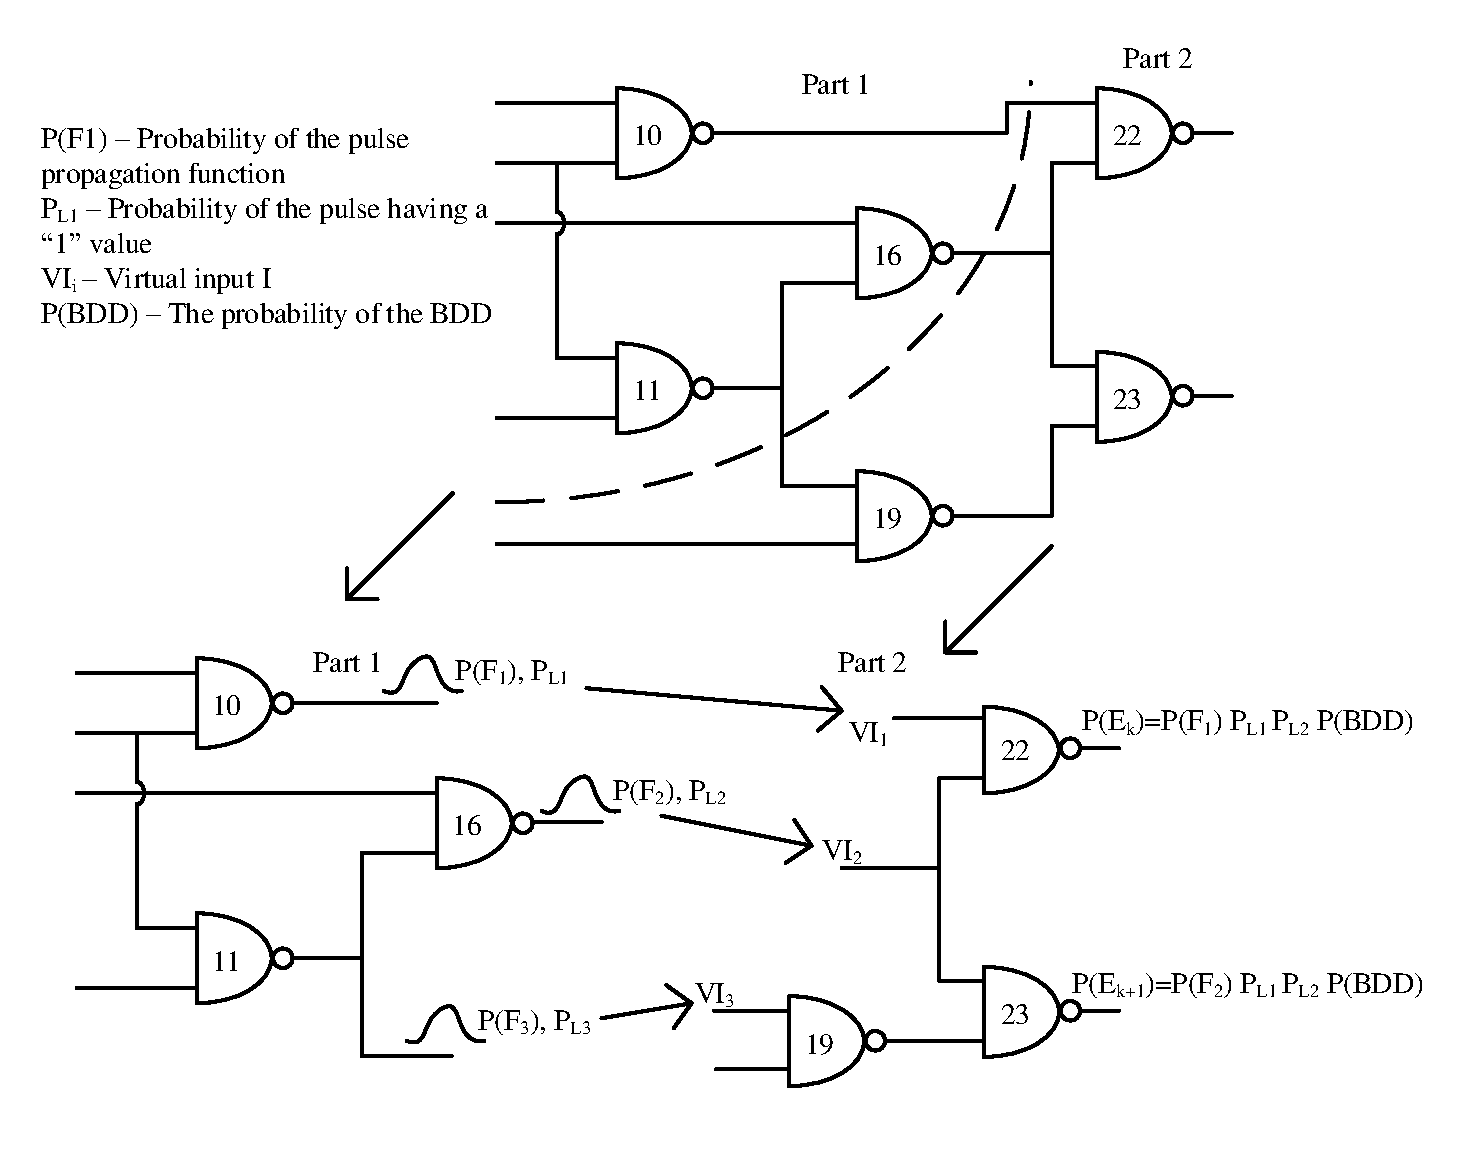
\includegraphics[width=\linewidth]{Figures/PartProp}
	%where an .eps filename suffix will be assumed under latex, 
	%and a .pdf suffix will be assumed for pdflatex; or what has been declared
	%via \DeclareGraphicsExtensions.
	\caption{Example of pulse propagation between partitions.}
	\label{PART_PROP}
\end{figure}

Lastly, when the simulator processes a circuit or partition output, the BDD functions for each pulse are solved to determine the probability. If the gate output is a primary output, the error probability for the gate is determined for each event $E_k$ using equation \ref{event_eq}. Additionally, if all other nodes have been visited, the MES is calculated using equation \ref{MES}. An overview of the whole simulation flow is given in Algorithm \ref{alg:fastmet}.

\begin{algorithm}
	\caption{FAST\_MET} \label{alg:fastmet}
	\begin{algorithmic} [1]
		\STATE Set Process Parameters
		\STATE Parse Netlist
		\STATE Organize Circuit Topologically
		\STATE Parse Circuit Into $k$ Parts
		\FOR{Each Partition}
		\STATE Extract Partition
		\STATE Set Virtual Inputs
		\FOR{Each Gate} 	
		\STATE Generate Pulse
		\STATE Generate Sensitization Function
		\STATE Propagate Pulse
		\STATE Calculate Convergence
		\IF{Primary Output}
		\STATE Calculate $P_{L,i}$
		\ELSIF{Edge of Partition}
		\STATE Solve BDD Probability
		\ENDIF
		\ENDFOR
		\ENDFOR		
	\end{algorithmic}
\end{algorithm}

\section{Results} \label{results}

The FAST\_MET simulator was tested on the ISCAS 85 combinational benchmark circuits. FAST\_MET was implemented in C++ on a machine with an eight core i7 and 16GB of RAM. The transistor look-up tables were characterized in HSPICE using the 32 nm Predictive Technology Model (PTM) \cite{PTM} where $V_{dd}$ was set to 1.05V. The unit gate capacitance was set to a constant capacitance of 2 fF to simulate the loading effects of the gates and interconnects. To calculate the MES, a single pulse with an energy of 15 fC was applied to each using the current equation in \cite{Ziegler1996} with $\tau$ being set to $32x10^{-15}$. It was assumed that each output is connected to a flip-flop implemented in the same process library with a setup time ($t_{setup}$) of 22 ps and a hold time ($t_{hold}$) of -7 ps in accordance to \cite{Nunes2013}. For all simulations, the probability of MET was set to 10\%. All METs were injected to a neighboring gate based on the netlist.

First, the accuracy of FAST\_MET without partitioning is compared to Monte Carlo simulation on c17 and c880 to ensure that the probabilistic functions provided exactly compute the logical masking effect. Larger circuits were not tested since they lead to long simulation times and lead to memory blow up for FAST\_MET without the use of partitioning. As can be observed in the Table \ref{table:MCvFAST}, FAST\_MET provides exact estimation of the output error with an over 5x speedup.

\begin{table}[ht]
	\begin{center}
		\caption{Comparision of FAST\_MET vs Monte Carlo}
		\label{table:MCvFAST}
		\begin{tabular}{|c|c|c|c|}
			\hline
			Circuit& Simulator & MES & Run Time\\ 
			\hline
			c17 & Monte Carlo & $3.92x10^{-4}$ & 0.429\\
			\hline
			c880 & Monte Carlo & $4.15x10^{-4}$ & 9110.35\\
			\hline
			c17 & FAST\_MET & $3.92x10^{-4}$ & 0.0974\\
			\hline
			c880 & FAST\_MET & $4.15x10^{-4}$ & 1909.37\\
			\hline
		\end{tabular}
	\end{center}
\end{table}

The FAST\_MET simulator provides an additional speedup through the use of partitioning. Table \ref{table:restable} provides the MES and the simulation time for various ISCAS 85 circuits while changing the partition size. According to the results, it shows that partitioning can provide an upward of 20X reduction in simulation time at a cost of accuracy compared to not using partitioning. Based off the results, it is shown that increasing the number of partitions follows the law of diminishing returns. For example in c880, the use of two partitions reduces the simulation time by 13X while the use of four partitions reduces the simulation time by 18X. While this is still a large decrease in simulation time, the error is increased by 4X. Additionally, it can be seen that in c17 the use of partitioning actually increases the simulation time. This is due to the time to simulate the circuit is less than the overhead incurred by the partitioning algorithm.

As observed by the results, the proper partition size to ensure an optimal trade-off between error and simulation time can be determined. For the current implementation, each partition was balanced based on the number of fan-in nodes to the gates. This is based on the assumption that gates with more fan-in nodes have a higher computational complexity due to more convergence cases and larger BDD sizes. To provide some direction on the ideal partition size, the average number of fan-in nodes among all partitions were counted and provided in Table \ref{table:restable}. For circuits c880 and c1355, the optimal trade-off between the error and simulation time was at a partition size of three hundred fan-in pins. On c1355, for example, the error between the MES for one partition (ideal) and the partitioned circuit for two and four partitions is $0.42x10^{-5}$ and $0.47x10^{-5}$ respectively. While the difference in error is very small, the simulation time is halved when four partitions are used. 

\begin{table}[ht]
	\begin{center}
		\caption{FAST\_MET Performance vs Number of Partitions}
		\label{table:restable}
		\begin{tabular}{|c|c|c|c|c|}
			\hline
			Circuit& Parts & MES & Run Time & Partition Size\\ 
			\hline
			c17 & 1 & $3.92x10^{-4}$ & 0.0974 & 12\\
			\hline
			c17 & 2 & $3.83x10^{-4}$ & 0.1377 & 6\\
			\hline
			c880 & 1 & $4.15x10^{-4}$ & 1909.37 & 729\\
			\hline
			c880 & 2 & $3.13x10^{-4}$ & 139.54 & 350\\
			\hline
			c880 & 4 & $8.37x10^{-4}$ & 107.72 & 180\\
			\hline
			c1355 & 1 & $2.38x10^{-4}$ & 3685.00 & 1064\\
			\hline
			c1355 & 2 & $1.96x10^{-4}$ & 459.00 & 536\\
			\hline
			c1355 & 4 & $2.85x10^{-4}$ & 242.60 & 270\\
			\hline
			c1355 & 8 & $3.67x10^{-4}$ & 167.961 & 135\\
			\hline
		\end{tabular}
	\end{center}
\end{table}

\section{Conclusion} \label{conc}
In this paper, the FAST\_MET simulator is proposed. First, probabilistic equations were provided which allow for accurate consideration of the propagation effects of METs. In addition to the accurate approximation of the logical masking effect, FAST\_MET uses a SPICE-like accurate electrical masking model. In the results it was shown that the tool provides a good trade-off between simulation time and accuracy due to the use of partitioning and an accurate masking model. Additionally, it is shown that the number of partitions reduces the simulation time up 18x compared to not using partitioning and 90x compared to Monte Carlo simulation.

% use section* for acknowledgement
%\section*{Acknowledgment}

\bibliographystyle{plain}
\bibliography{Bibfile}

\end{document}


